\documentclass[12pt]{article}

% Packages
\usepackage{lastpage} 
\usepackage{fancyhdr}	%For header and footer
\usepackage{amsmath, amsthm, amssymb} %For mathematics
\usepackage{graphicx}
\usepackage{hyperref}	%For hyperlinks

% Page setup
\setlength{\topmargin}{-0.4in}
\setlength{\topskip}{0.3in}    % between header and text
\setlength{\textheight}{9.in} % height of main text
\setlength{\textwidth}{6.5in}    % width of text
\setlength{\oddsidemargin}{0in} % odd page left margin
\setlength{\evensidemargin}{0in} % even page left margin
\setlength{\parindent}{0pt}	% Suppress the indent

% Macros
\newcommand*{\bv}[1]{\textbf{#1}} % Write vectors in bold case within an equation environment

% Header and Footer
\pagestyle{fancy}%\fancyhead{}
\fancyhf{}	% Clear the default header and footer
\fancyhead[L]{MAE 3195 \\ Name:}
\fancyhead[R]{Credit Sheet 3 \\ \thepage /\pageref{LastPage}}


% Title
\title{MAE 3195, Credit Sheet 3, Tutorial Lesson 3\\
Creating a Simple Object (Part II)}
\date{}

% Body of document
\begin{document}
\maketitle

For this homework, read and work through Lesson 3 in your text \textit{ProEngineer Tutorial}. Before you launch Pro/E, make a new sub-directory in your personal MAE3195 directory titled ``HW3''. Copy the latest revision of ``***-hw2.prt'' in your HW2 folder, and then paste a copy in your HW3 folder. The latest revision of the ``***-hw2.prt'' is indicated by the highest suffix in the filename (e.g. rrv-hw2.prt.5 is revision 5 and a later revision than a file named rrv-hw2.prt.4). Be sure not to cut and paste because you want to leave a copy of your work in the HW2 folder. After pasting ``***-hw2.prt'' into the HW3 folder, rename the file to ``***-hw3.prt.*''.\\

Launch Pro/E and immediately set/verify that your working directory is set to HW3. When your textbook tells you to retrieve the file from Lesson 2, be sure to select your ``***-hw3.prt'' file that is now stored in HW3. If you correctly set your working directly to HW3 folder, then HW3 folder should be the default folder after selecting File$>$Open. Proceed with the remainder of Lesson 3 as described in the textbook.\\

Since this is a tutorial homework, each individual must perform this work independently. You are encouraged, however, to discuss the assignment with other students as necessary.\\

It is recommended (but not required) that you study the ``Questions for Review'' and create some of the ``Exercise'' models at the end of the chapter. After completing the lesson, answer the following questions and bring this Credit Sheet with you to class on the due date.

\section*{Review Questions}
\begin{enumerate}
	\item What is the difference between the terms ``protrusion'' and ``extrusion''?
	\pagebreak %\vspace{1.in}
	\item Once a feature has been created, describe two methods for changing its dimensions.
	\vspace{1.25in}
	\item Describe what is meant by design intent.
	\vspace{1.25in}
	\item Describe the various techniques for capturing design intent within a 2D sketch.
	\vspace{1.25in}
	\item On the back of this sheet, sketch two copies of the 2D sketch necessary to create the geometry shown in fig.~\ref{figQuestion5}. Include lines and a rectangle that illustrate the three default datum planes as they would appear in sketch mode. Place dimensions on your sketches that illustrate two alternative dimension schemes that will exactly constrain (no over or under constraint) the size and shape of the 2D sketch.
\end{enumerate}

\begin{figure}[h!]
  \begin{center}
    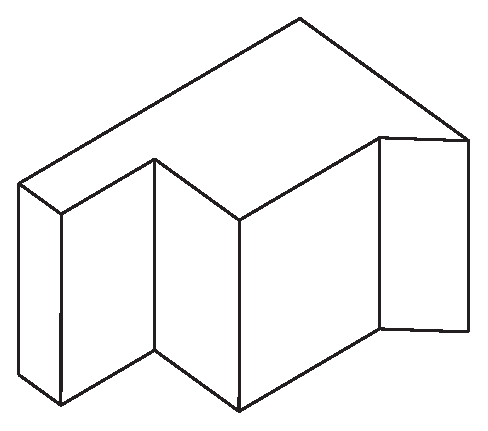
\includegraphics[width=2.in]{mb_CS3_question5}
    \caption{Geometry for question 5}
    \label{figQuestion5}
  \end{center}
\end{figure}

\end{document}